%!TEX root = thesis.tex

%:-------------------------- Preamble -----------------------

% Three languages are supported, which will be reflected in the logo on the front page. Pass the appropriate language
% specified as a class option to uit-thesis. Passing any other languages supported by babel will result in the default
% language on the frontpage. If no language is passed, the default is selected.
%  - USenglish (default)
%  - norsk
%  - samin
% The frontpage comes in two variants, Master's thesis and PhD. Master is default, use classoption 'phd' for the PhD version.
\documentclass[USenglish]{uit-thesis}

% Lorem ipsum
\usepackage{lipsum}

\makeglossaries

% Add external glossaryentries
\loadglsentries{acronyms}
\newacronym{api}{API}{application programming interface}\glsunset{api}
\newacronym{2api}{2API}{application programming interface}
\newacronym{d3}{D3}{Data-Driven Documents}
\newacronym{camilla}{CAMILLA}{Camilla is cool!!}
\newacronym{html5}{HTML5}{version 5 of the HyperText Markup Language standard}
\newglossaryentry{thesis}
{
  name=thesis,
  description={is a document submitted in support of candidature for an
    academic degree or professional qualification presenting the author's
    research and findings
    },
}
\newglossaryentry{lage}
{
  name={long ass glossary entry},
  description={is a long ass entry with a lot of text describing the properties of the glossary entry. Hopefully this spans some lines now.
  },
}


\newcommand{\listdefinitionname}{My list of definitions}
\newlistof{definition}{def}{\listdefinitionname}
\newcommand{\definition}[1]{%
  \refstepcounter{definition}%
  \par\noindent\textbf{The Definition~\thedefinition. #1}%
  \addcontentsline{def}{definition}
    {\protect\numberline{\thechapter.\thedefinition}#1}\par%
}

\begin{document}

%:-------------------------- Frontpage ------------------------

\title{From Physical to Virtual Sensors (PVS)}
%\subtitle{Subtitle}			% Optional
\author{Camilla Stormoen}
\thesisfaculty{Faculty of Science and Technology \\ Department of Computer Science}
\thesisprogramme{INF-3983 Capstone Project in Computer Science … December 2017}
%\ThesisFrontpageImage{example_image.jpg}	% Optional

\maketitle

%:-------------------------- Frontmatter -----------------------
\frontmatter

%\begin{dedication}
%To somebody.

%Fuck you very much.
%\end{dedication}

%\begin{epigraph}
%\epigraphitem{Simplicity is prerequisite for reliability.}{Edsger Dijkstra}
%\epigraphitem{Beware of bugs in the above code;\\I have only proved it correct, not tried it.}{Donald Knuth}
%\end{epigraph}

\begin{abstract}
%\lipsum[2-3]
\begin{description}
\item[W3] Whats wrong with the world? / motivation 1-3 setninger
\item[Architecture - 1-3 setninger]
\item [Design- 1-3 setninger]
\item[Implementation - 1-3 setninger]
\item[Experiments - 1-3 setninger]
\item[Results - 1-3 setninger]
\item[Lessons learned/main conclusion - 1-3 setninger]
\item [Kutt heller etterpaa] 
\end{description}

This dissertation present/describe ...
\end{abstract}


%\begin{acknowledgement}
%\lipsum[4-8]
%\end{acknowledgement}

\tableofcontents

%\listofdefinition
\listoffigures

%:-------------------------- Mainmatter -----------------------
\mainmatter

\chapter{Introduction}
\begin{itemize}
\item Mention focus on camera-sensors/data, and not other sensors?!
\textit{John M.: Hvorfor fokus på bilder - forenkle, begrense, starte et sted}
\item Talk a little bit about COAT in general?
\end{itemize}

This project will develop an abstraction for virtual sensors, and do a prototype of the abstraction on a set of computers with physical sensors.

The purpose is to provide for a more powerful and flexible sensor in the COAT monitoring of the arctic tundra. As such, a fox feeding station is the usage domain to be used for the prototype.



%There are increasing numbers of physical sensors used for various purposes. For example, ...

%OTTO RETTING: Assume biologists want to search for pictures of a specific animal from different locations in the Arctic Tundra. A virtual sensor would collect/\textbf{locate} data from the physical/\textbf{storage} sensors and then return those images that matches to the biologists request.

\section{Motivation}
The motivation!
\begin{itemize}
\item W3
\item Problem definition: This project investigated ... x, with the purpose of y.
\end{itemize}

The motivation  behind this project is that no single sensor may cover the sensing needs, and that sensing needs can change rapidly over time. Consequently, there is a need for sensor fusion, and allow for combining sensors at different computers.

\section{Contributions}
What was the contribution?
%OTTO: Principles, models, artifact and evaluation of it. Lessons learned/insights. Conclusion

\section{Assumptions}
AVGRENSE, VIKTIG!!
Something about motivation and stuff

\section{Limitations}
AVGRENSE, VIKTIG!!

\begin{itemize}
\item Mention focus on camera-sensors/data, and not other sensors?!
\end{itemize}

%\begin{itemize}
%\item The first item .
%\end{itemize}

%\begin{enumerate}
%\item The first item
%\end{enumerate}

%\begin{description}
%\item[Entry A] with definition A.
%\end{description}

%\newpage

\iffalse
\subsection{A subsection - example}
We can use the \ac{api} to \ac{2api} do stuff, and write about what we did in a \gls{thesis}!

This is some stuff, {\sc smallcaps {\em smallcapsemphasized}} {\em regularemphasized}

\Gls{lage}: a test glossary entry.

If the acronym \ac{uit} is displayed, then loadglsentries works.
Hello. This is a test: \ac{camilla}

It is fun to use modern \upsc{OpenMP} technology!\footnote{This is a snarky footnote. Words and etc. Semantic web technologies are technologies that enable semantification of the Web as we know it today. Hopefully this spans some lines now.}

It is fun to use \emph{modern \upsc{OpenMP}} technology! And it is fun to use \ac{d3} and \ac{html5}.

Referencing figure \ref{fig:ex} to test link.\footnote{This is another
footnote.}

\definition{Some other definition}
\fi




\chapter{Related Work}
\iffalse
\begin{itemize}
\item Taking Sensor Networks from the Lab to the Jungle
\item Wireless Sensor Networks for Habitat Monitoring
\item Building Virtual Sensors and Actuators over Logical Neighborhoods
\item A virtual sensor system for user-generated, real-time environmental data products
\item Integrating modeling and smart sensors for environmental and human health
\item Capability representation model for heterogeneous remote sensing sensors: Case study on soil moisture monitoring
\item Dice: Monitoring Global Invariants with Wireless Sensor Networks 
\\ \em{Ştefan Gună, Luca Mottola, and Gian Pietro Picco. 2014. DICE: Monitoring global invariants with wireless
sensor networks. ACM Trans. Sensor Netw. 10, 4, Article 54 (April 2014), 34 pages.}
DOI: http://dx.doi.org/10.1145/2509434
\textit{Guna:2014:DMG:2633905.2509434,
 author = {Gun\u{a}, \c{S}tefan and Mottola, Luca and Picco, Gian Pietro},
 title = {DICE: Monitoring Global Invariants with Wireless Sensor Networks},
 journal = {ACM Trans. Sen. Netw.},
 issue_date = {June 2014},
 volume = {10},
 number = {4},
 month = jun
 pages = {54:1--54:34},
 articleno = {54},
 numpages = {34},
 url = {http://doi.acm.org/10.1145/2509434},
 doi = {10.1145/2509434},
 publisher = {ACM}}
\end{itemize}
\fi

\section{Virtual Sensors}
A virtual sensor is a constructed sensor in contrary to a physical sensor \cite{VirtualSensors2006}. They are used in place of the real sensors where they read real physical sensor data and calculate the outputs by using some processing models.

Previous research have focused on simple in-network data aggregation techniques and the sensor networks are often represented as a database. Two examples of such approaches are TinyDB \cite{tinyDB} and Cougar \cite{cougar}, which enable applications to have a central point (base station) and create routing trees  to funnel replies back to this root. The main focus on these approaches are operating intelligent in-network aggregation and routing to reduce  the overall energy cost while still keep the semantic value of data high.
In both examples, the data aggregation is specified using an SQL-like language. However, queries cannot be used to merge different data types, only homogeneous data aggregation is achievable.
Their virtual sensors approach is  offering a simple interface and heterogeneous in-network data aggregation. Yet, our virtual sensors have no SQL-like language or a database to store the aggregated data. Our work also relies on physical sensor data which is already in a data storage, and not directly from the physical sensors.


A virtual node\cite{Ciciriello} is a set of physical sensors that a programmer can interact with as a single sensor. Their virtual nodes are implemented using TinyOS \cite{TinyOS} and their physical nodes are abstracted and specified using logical neighborhoods \cite{Mottola2006}\cite{Mottola2006_2}. The nodes are combined in a logical neighborhood that are specified based on their characteristics by the programmer. 


It is a prototype of a virtual sensor system for environmental observation with real-time customization of physical sensor data. 
The system can provide point-averaged radar-rainfall products at either temporal resolution of the radar or as a temporal average of a fixed time period, which is illustrated in Figure \ref{fig:rainfall_sensor}
In contrast, our virtual sensors system is running on-demand, not in real-time. \textbf{OGSÅ ANDRE ULIKHETER}

\begin{figure}
\centering
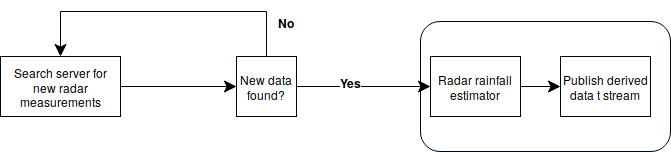
\includegraphics[width=\textwidth]{rainfall_sensor.png}
\caption{Figure illustrating the virtual rainfall sensor.}
\label{fig:rainfall_sensor}
\end{figure}


%\subsection{dice - expand!}
%Dice??
%\textit{"Improve network lifetime -> routing protocol for many-2-many communication". Talking about TinyOS and CTP.
%In this article we present DICE, a system enabling WSN-based distributed monitoring of global invariants. A DICE invariant is expressed by predicates defined over the state of multiple WSN nodes, such as the expected state of actuators based on given sensed environmental conditions.}

%\textit{We presented DICE (Distributed Invariant CheckEr), a system for WSN-based distributed monitoring of global invariants in physical processes. DICE provides a declarative language to specify invariants and a runtime support enabling efficient monitoring of their violations.}

%\textit{\textbf{SYSTEM ARCHITECTURE}
%We describe the toolchain and runtime architecture of DICE. Our prototype targets TinyOS [Hill et al. 2000], and relies on CTP [Gnawali et al. 2009 - Collection tree protocol: two principles of wireless routing protocols] for the tree-based forwarding necessary to the TREE dissemination strategy. Nevertheless, the techniques we describe do not depend on either.
%We use our TinyOS implementation of DICE, described in Section 4, to run both simulation and tested experiments.
%In computer science, an invariant is a condition that can be relied upon to be true during execution of a program, or during some portion of it. It is a logical assertion that is held to always be true during a certain phase of execution.}


%\textit{\textbf{Sensor-Cloud Infrastructure}
%Physical Sensor Management with Virtualized Sensors on Cloud Computing
%http://ieeexplore.ieee.org/document/5635688/\#}





\chapter{The Dataset} \label{chap:data_set}
\textbf{HVORDAN DE ER SAMLET, HVORDAN DE ER ORGANISERT?}

The dataset is provided by COAT and contains over 1.6 millions of pictures taken from 2011 to 2015 by their camera traps stationed in the Arctic Tundra in Finnmark, Norway. The camera traps are placed at six different areas in the Arctic Tundra: Nordkynn, Ifjord, Komag, Nyborg, Stjernevann and Gaissene.
The dataset contains pictures during night- and daytime. The cameras have infrared flash so the cameras can take pictures at nighttime. These pictures are without color while the pictures taken at daytime are with color, as shown in Figure \ref{fig:pictures}.


\begin{figure*}[t!]
    \centering
    \begin{subfigure}[t]{0.5\textwidth}
        %\centering
        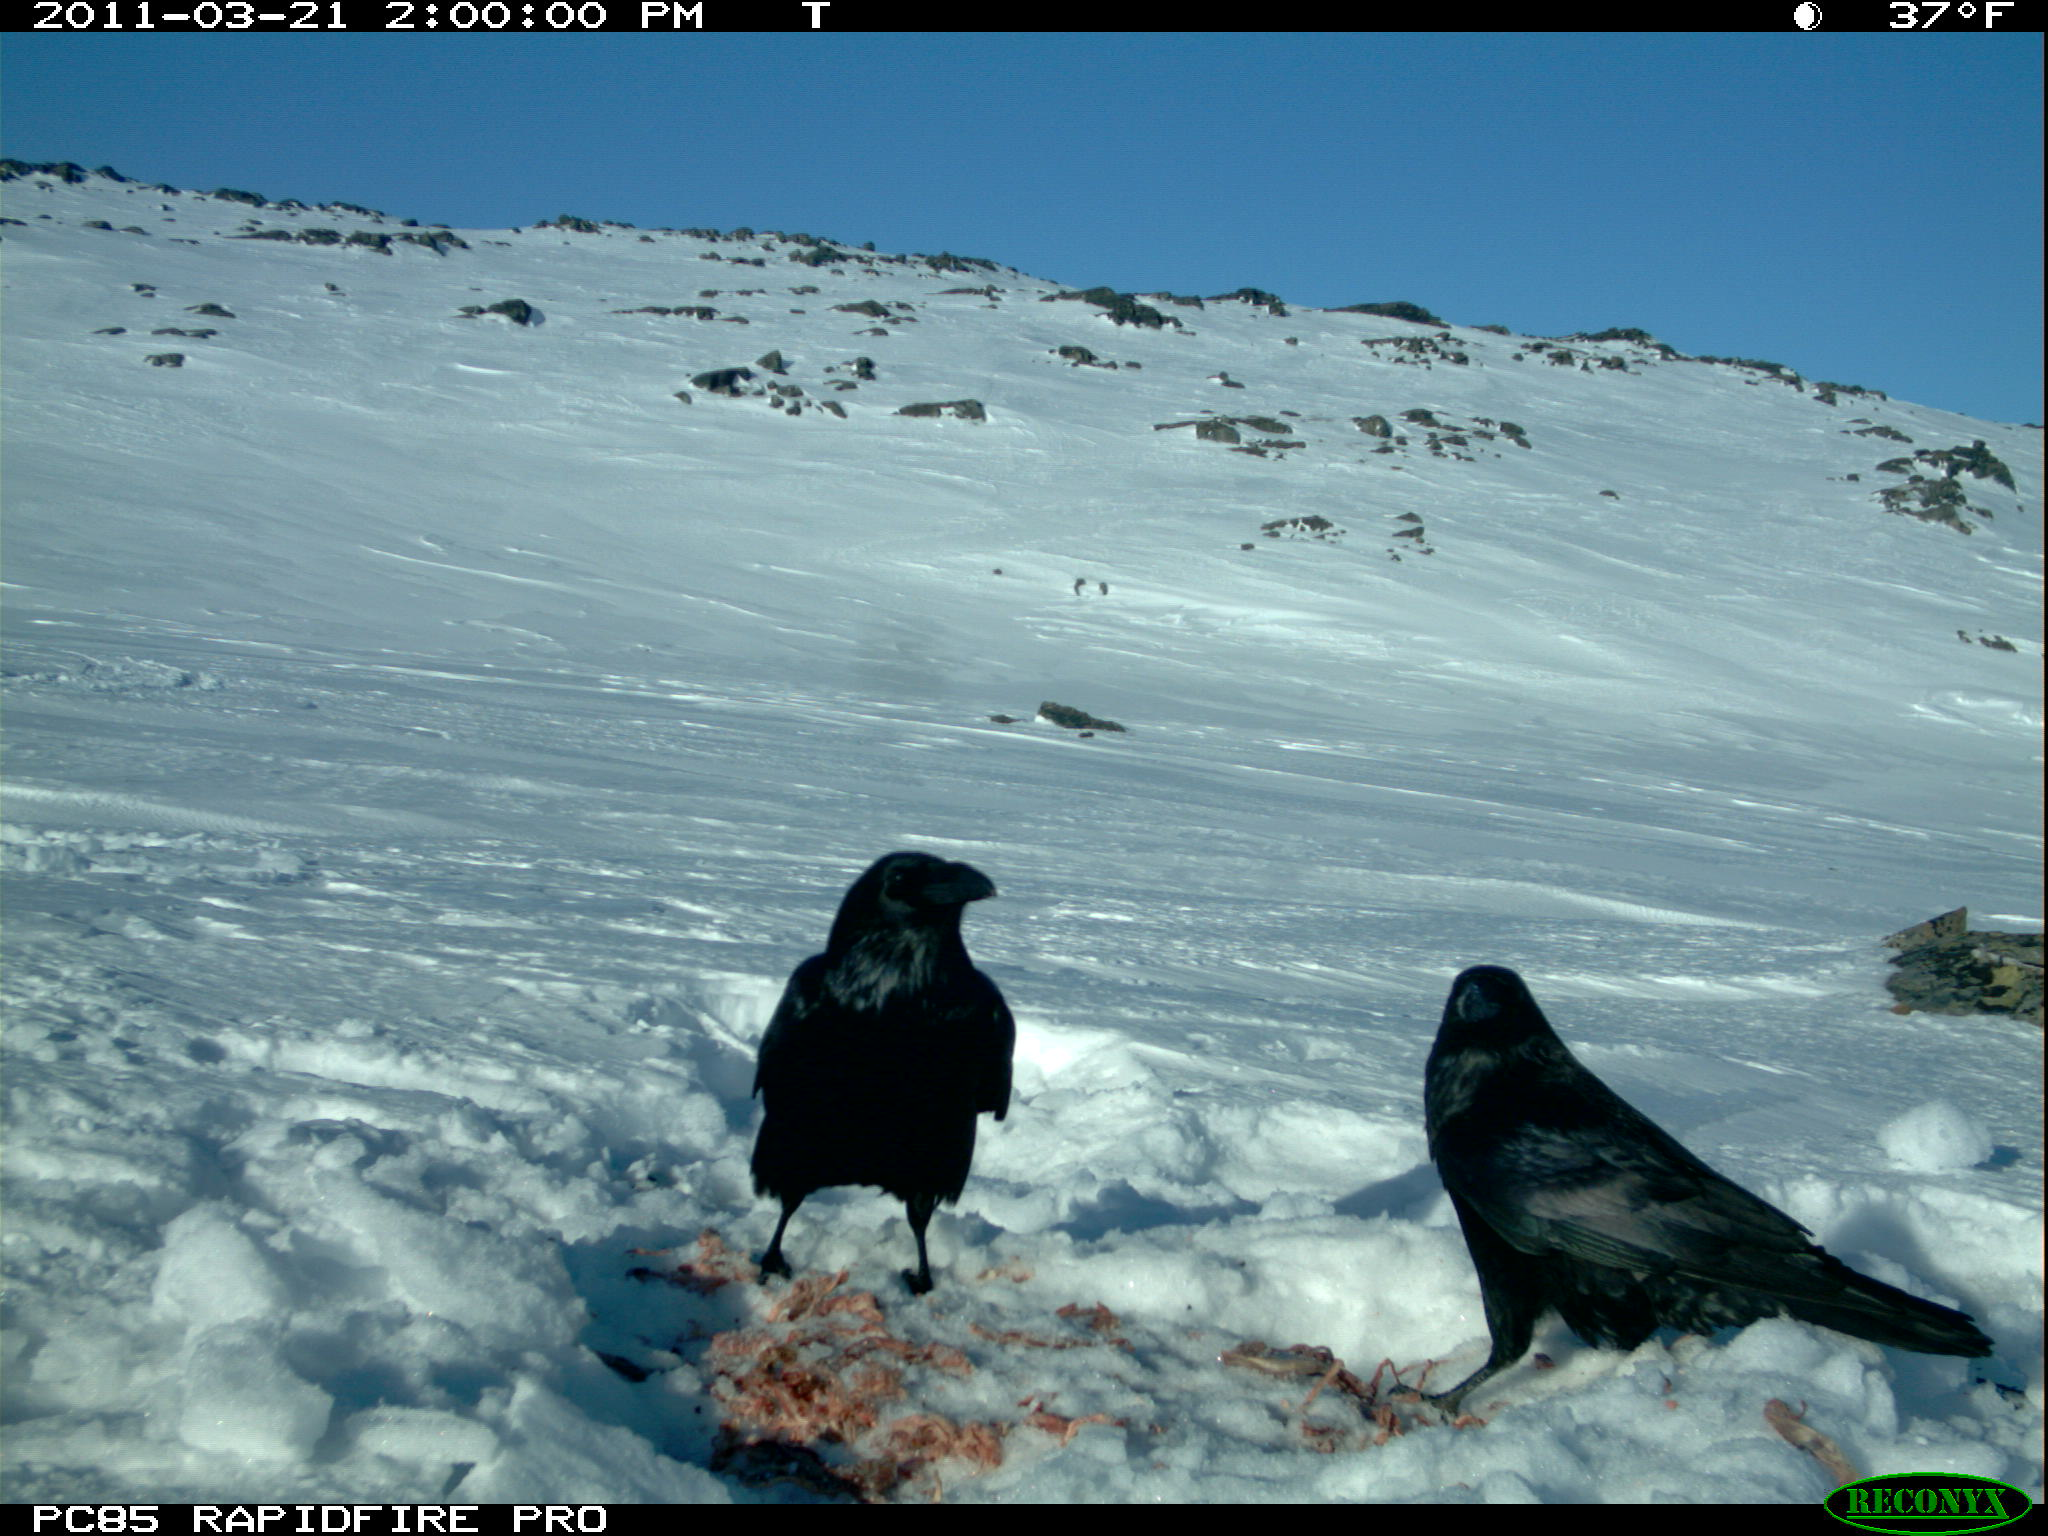
\includegraphics[width=\textwidth]{IMG_0040.JPG}
        \caption{Picture of ravens at daytime.}
    \end{subfigure}%
    ~ 
    \begin{subfigure}[t]{0.5\textwidth}
        %\centering
        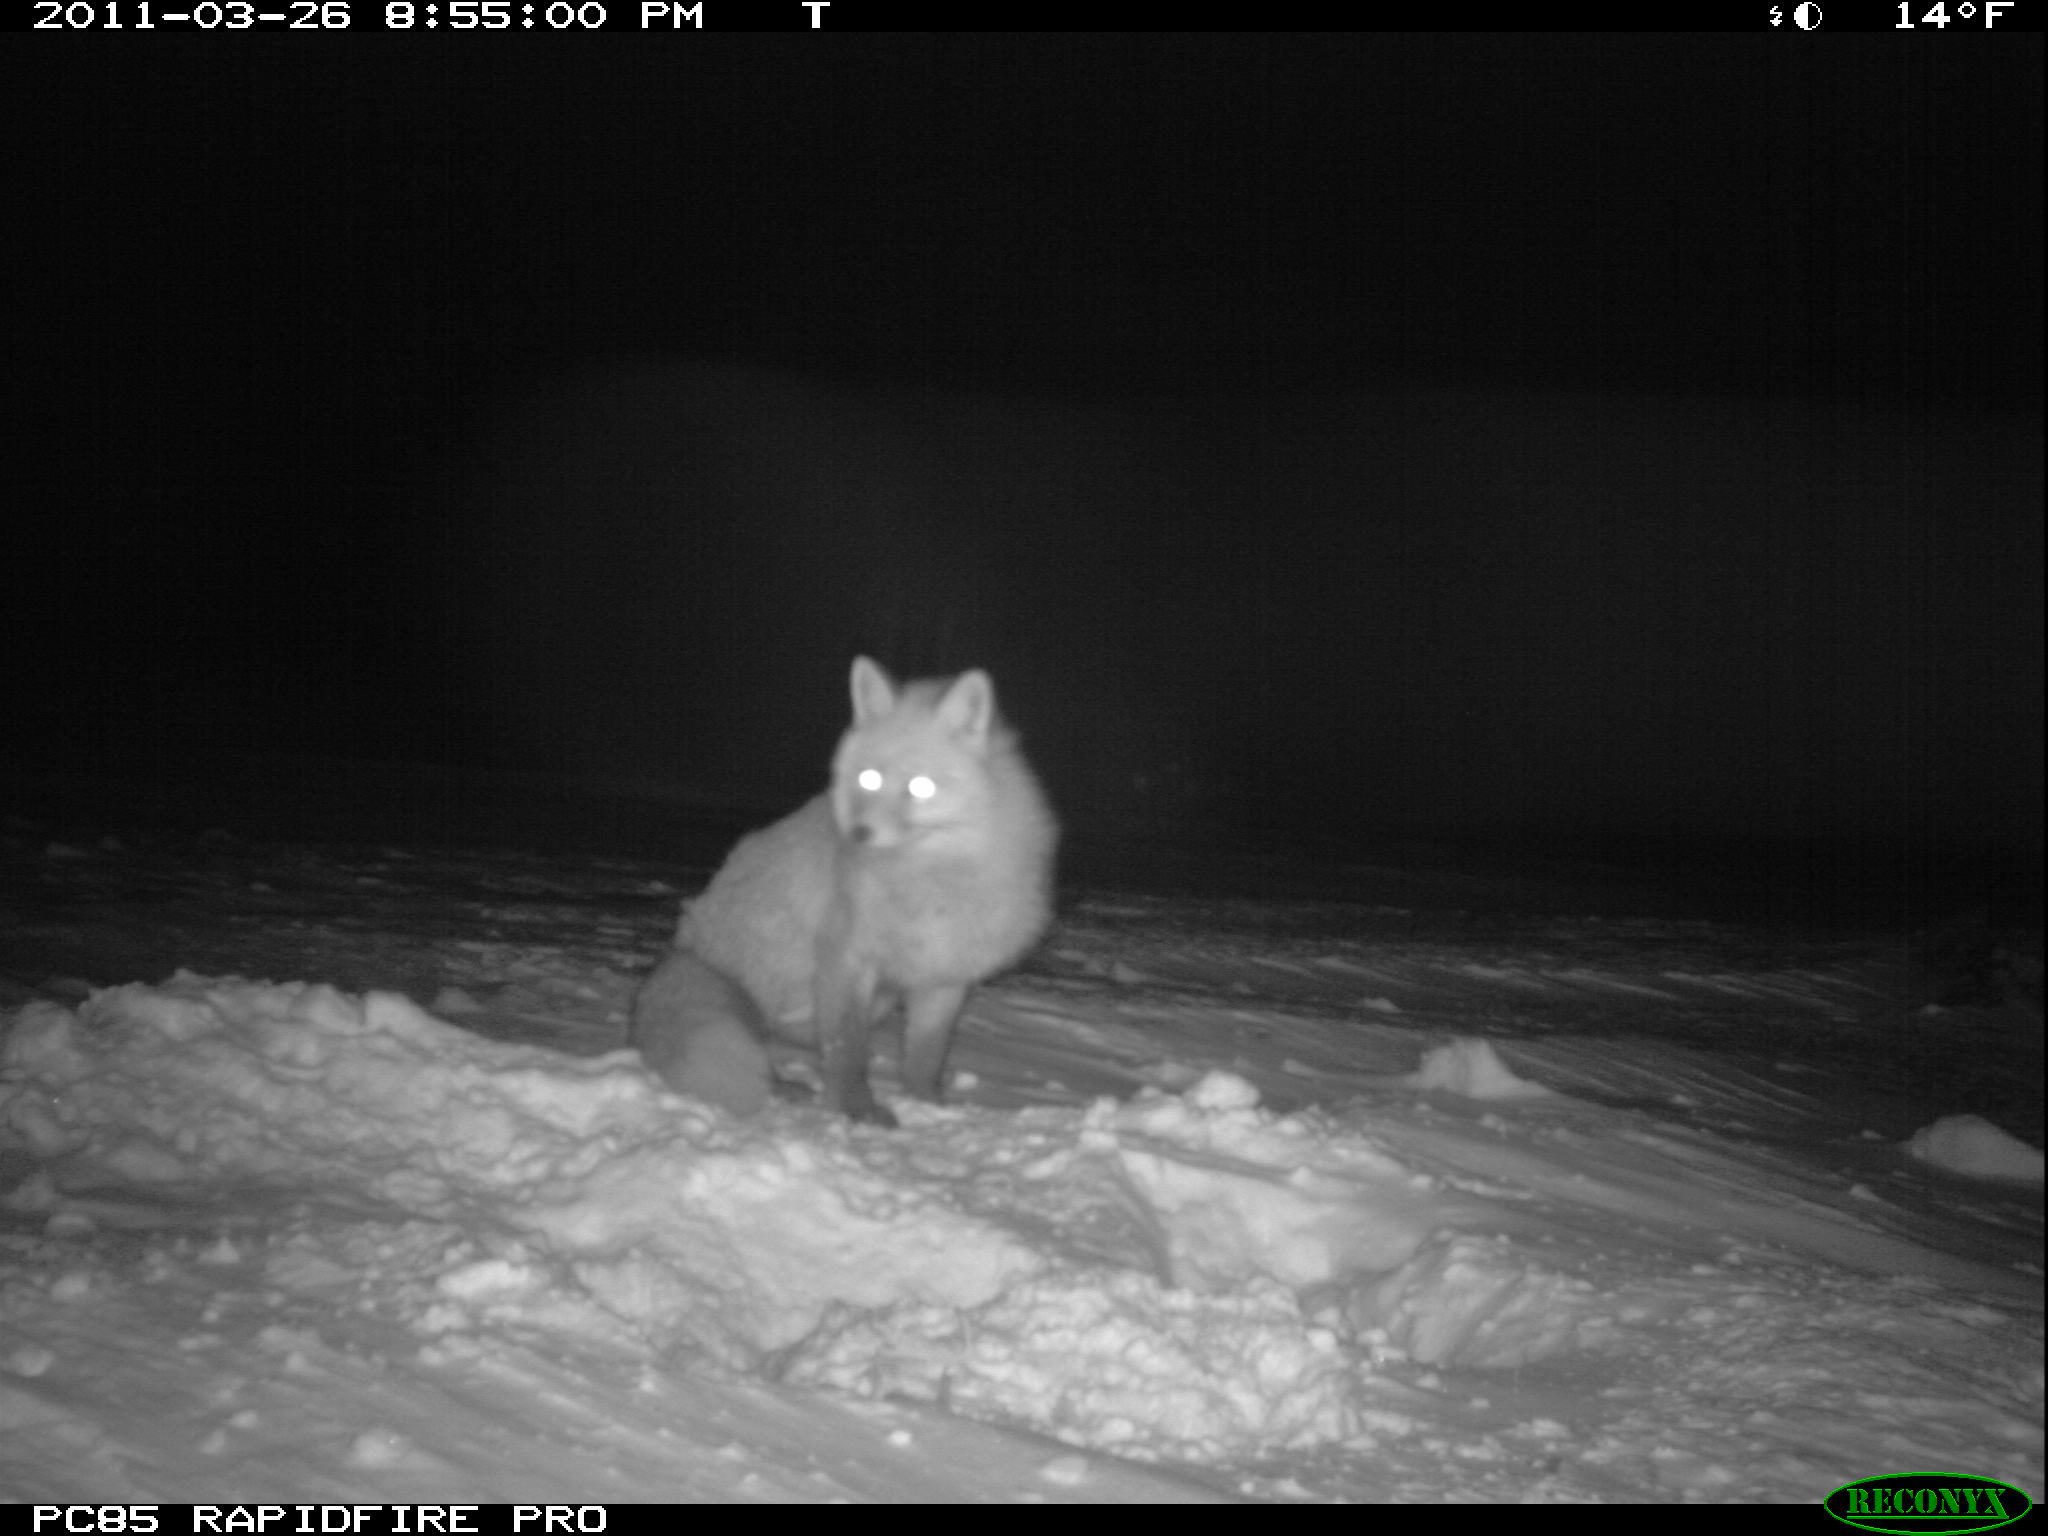
\includegraphics[width=\textwidth]{IMG_1562.JPG}
        \caption{Picture of an arctic fox at nighttime.}
    \end{subfigure}
    \caption{Images from the COAT dataset showing how a picture can contain colors or greyscale.}
    \label{fig:pictures}
\end{figure*}


\section{Dataset Directory Structure}
The pictures in the dataset is structured in directories and folders. The dataset is first divided into different years going from 2011 to 2015. Each of these folders are then again divided into the area of the 5 camera traps in the Arctic Tundra. Inside each of these folders specified by the area, they contain folders from each site inside the specific area.
Figure \ref{fig:directories} shows a cropped screenshot of the directories.

%\textbf{(In total 1976 directories.) -- mappestruktur -- metadata på bilder}

\begin{figure}
\centering
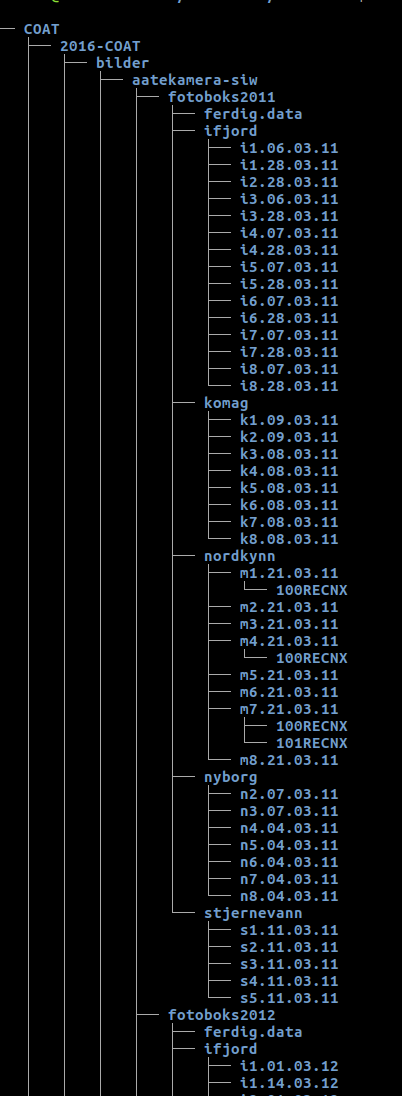
\includegraphics[scale=0.5]{directory.png}
\caption{Figure showing a cropped screenshot of the structure of the directories.}
\label{fig:directories}
\end{figure}


COAT also provided excel-sheets with information about all of the images in the dataset. The dataset contains the images metadata and animal classification, but did not contain any filenames or a filepath. We then had to find a method to find out which images correspond to the metadata in the excel-sheets. Fortunately, each image had metadata stored in Exchangeable Image File Format (EXIF). We recursively traverse the directories where images are located and read date-time from the metadata and store it in a dictionary with date-time as key and image-path as value. This was quite a time-consuming task because of the number of images to process.


\chapter{Architecture}
This chapter describes the architecture of the system.
There are 6 components in the system: physical sensors, \textit{raw data, anaytics and classified data} storage, fusion of data, fused data, virtual sensors and the user interface. 

The architecture of the system is presented in Figure \ref{fig:architecture}. The arrows indicates the communication lines and the dataflow between each component in the system. \textbf{..eller flyten av data/dataflow eller hvem som er aktiv i å gjøre akses/sende - NOE SÅNT HER OGSÅ I NY FIGUR}

\begin{figure}
\centering
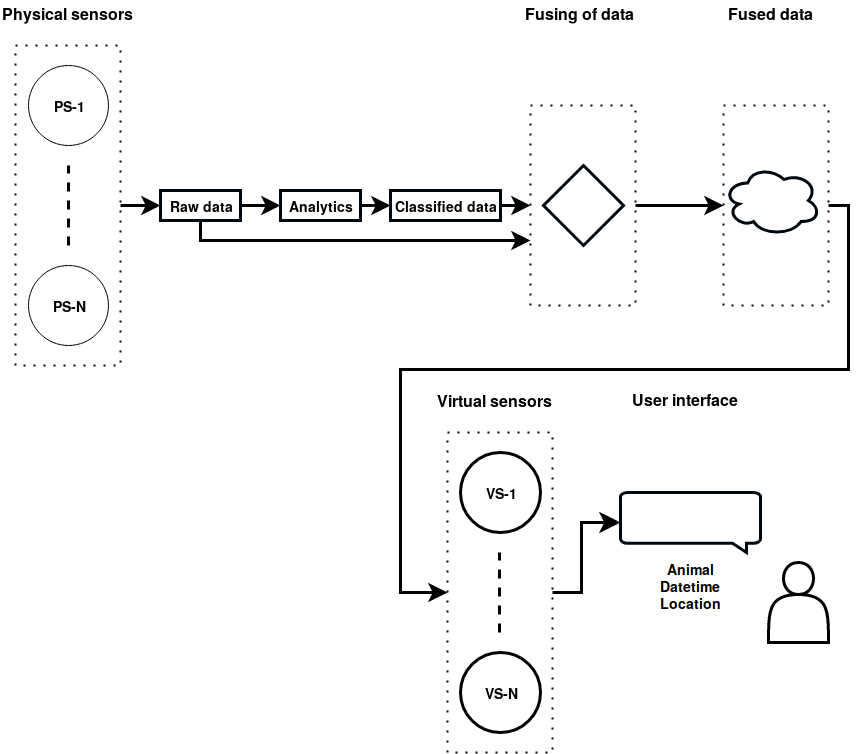
\includegraphics[width=\textwidth]{Architecture_otto4.png}
\caption{Figure showing the system architecture.}
\label{fig:architecture}
\end{figure}

\begin{figure}
\centering
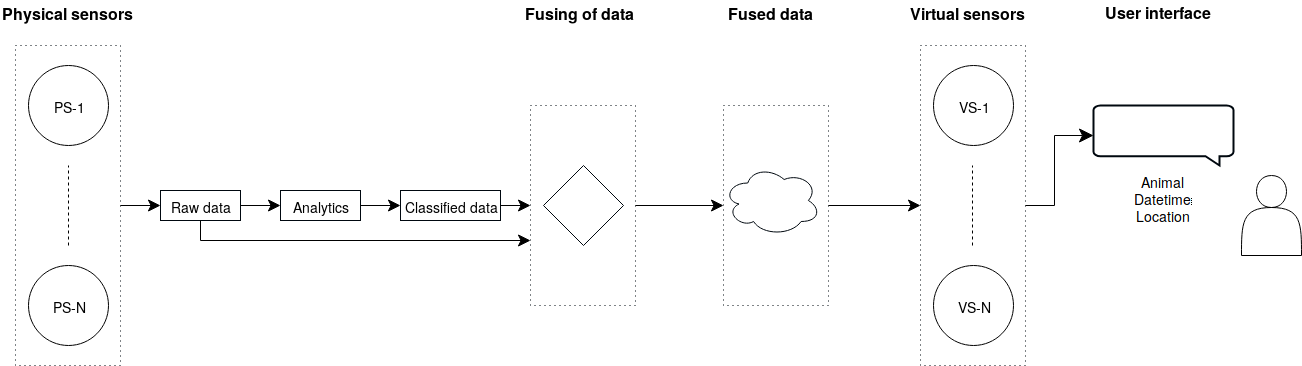
\includegraphics[width=\textwidth]{Architecture_otto.png}
\caption{Figure showing the system architecture.}
\label{fig:architecture}
\end{figure}

\section{Physical Sensors}
The physical sensors produce raw data. The raw data consists of images from different bait-camera sensors.
The data also contains metadata about each image, as described in Chapter \ref{chap:data_set}. 

(\textbf{More on the metadata!) --- ha det i Chapter \ref{chap:data_set} med dataset???}


\section{Raw Data}
Raw data from physical sensors..

\section{Analytics and Classified Data}
Biologist have detected animals in each picture and made excel-files containing metadata about each picture.(ELLER NEVNE DETTE I CHAPTER DATASET??

\section{Fusing of data and Fused Data}
\subsection{Fusing of data}
Get analytics and classified data from raw data (excel) and the raw-data and fuse/aggregate correlated/corresponding(?) data.


\subsection{Fused Data}
The fused data retrieves it's data and on demand. The fused data is the physical sensors location combined with necessary metadata such as date-time, location, site, year, what kind of animal there as in the image and also how many animals there was/\textbf{and animal classification}.


\section{Virtual Sensors} \label{sec:arch_vs}
The virtual sensors are divided into multiple sensors representing different animals that scientists are interested in, like ravens, red foxes, golden eagles or polar foxes.
These virtual sensors 

The user types in the user interface, described in Section \ref{sec:arch_user_int}, what animal he/she wants to see, where it is and the date-time and the search is redirected to the sensor related to that specific animal. The virtual sensor retrieves its result from the fused data.

\textbf{UTDYP "QUERY" SPRÅKET og UTDYP DE VIRTUELLE SENSORENE}

\subsection{Raven Sensor, Red Fox Sensor, Golden Eagle Sensor, no-animal sensor}
\textit{Eller ha disse som eget kapittel "My virtual sensors".. Tror jeg utdyper mer her ettersom VS er helt like bortsett fra at de avhenger av hva slag dyr man er ute etter..}


\section{User Interface} \label{sec:arch_user_int}
A user wants to retrieve fused data about animals. The user interacts with the virtual sensor user interface. This takes care of the interaction with the virtual sensor. When a user gives a command, the responsible virtual sensor retrieve data from the fused data as described in the section above/Section \ref{sec:arch_vs} , and presents the result back to the user.



\chapter{Design}
Client/Server, p2p, put/get, pub/sub, protokoller, FTP etc..
BESKRIV INTERAKSJONEN MELLOM ENHETENE!!

Virtual sensors probably uavhengige prosesser, ikke threads ettersom man evt vil addere flere sensorer og unnga a starte alle sensorer på nytt igjen..
Er de virtuelle sensorene servere eller client/publisher?

In this chapter we will look at the design of the system and present the design of each component of the architecture. Figure \ref{fig:design} shows the design of the system. The arrows indicates the communication lines. The dotted arrows show how the data storage is structured with files and pictures. \textbf{Få med direction of arrows/active side?}

\ OLD
\textit{In this chapter we will look at the design of the environment. We will present the design of the data storage, the fused data the virtual sensors and the user application. Figure \ref{fig:design} shows the design of the system. The arrows indicates the communication lines. The dotted arrows show how the data storage is structured with files and pictures.}


\begin{figure}
\centering
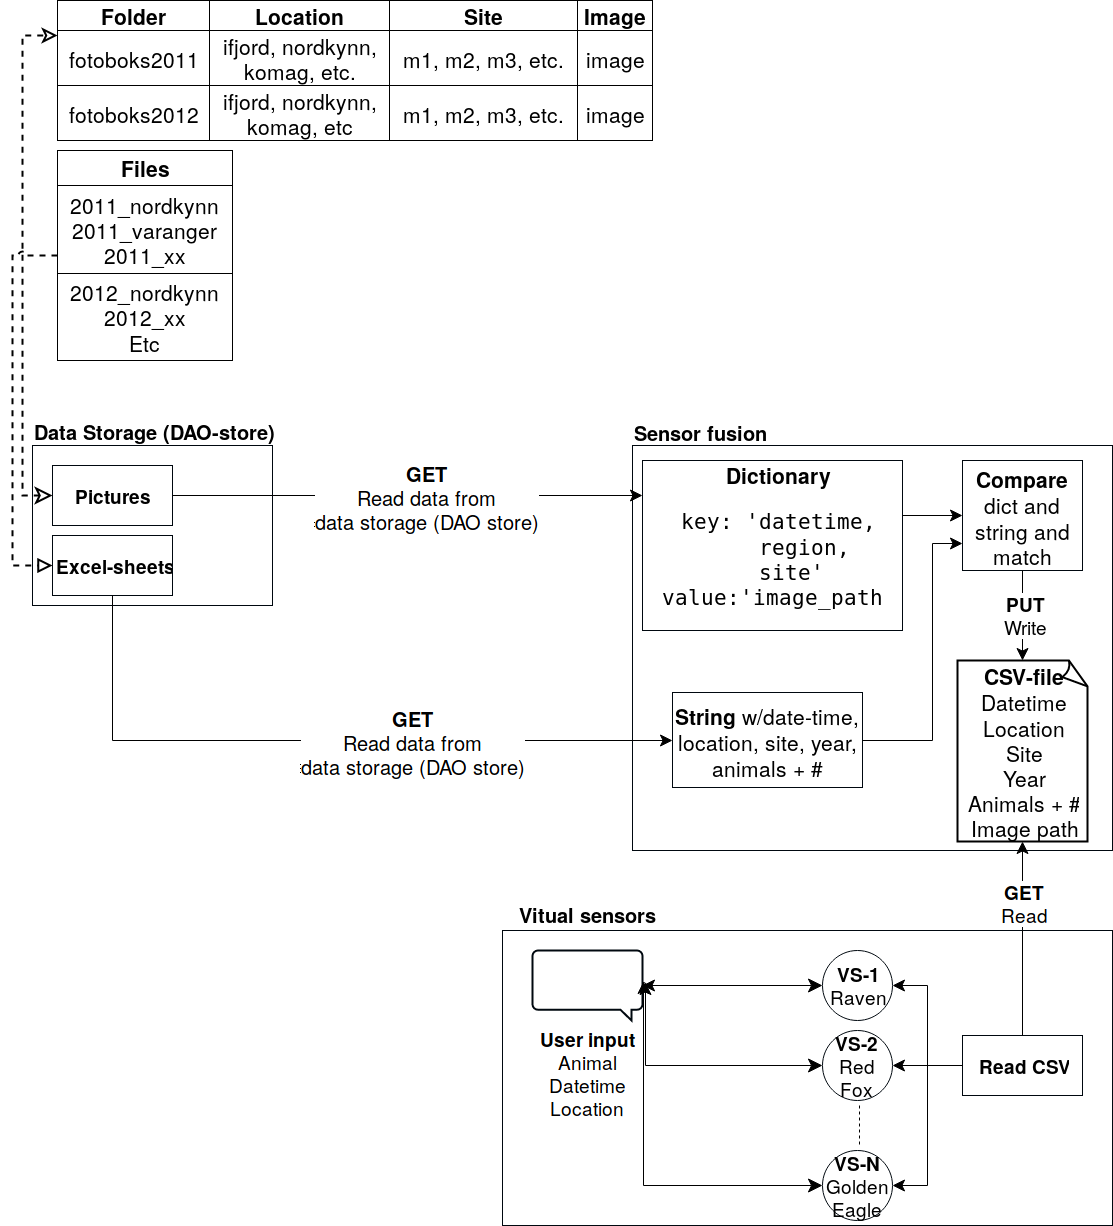
\includegraphics[width=\textwidth]{Design.png}
\caption{Figure showing the system design.}
\label{fig:design}
\end{figure}

\section{Data Storage} \label{ssec:des_fused}
%The dataset from the physical sensors contains over 1.6 millions of pictures from 2011 to 2016 taken from the Arctic Tundra in Finnmark, Norway. The physical sensors are placed at different areas in the Arctic Tundra such as Nordkynn, Komag, Nyborg, Stjernevann and Gaissene.
%The excel-sheets contains from 17 000 to 70 000 rows with information about each picture taken.

The excel-sheet in the data storage contains a pictures location, date-time, site, year and animal classification, but it did not contain any filename or a filepath. We then had to find a method to find out which images correspond to which field/row in the excel-sheet. Fortunately, each image had metadata stored in Exchangeable Image File Format (EXIF). We recursively traverse the directories where pictures are located and read date and time for each picture and store it in a Python dictionary, like a key-value store, with date and time as key and image-path as value. This was quite a time-consuming task because of the numbers of images to process.

... described in Chapter \ref{chap:data_set}...

%\section{Fused Data from Sensors}
%Rekursiv traversering av directories og leser metadata fra bildene (ca 1,6 mill bilder)) - Lagres i en dictionary hvor datetime og sted er key og image pathen er value).

%Disse sammenlignes og de som matcher blir skrevet til en CSV-fil.

\section{Virtual Sensors TIL Sensor Fusion}
The respective virtual sensor must handle events from the user. Assume a user wants to find pictures of a red fox at a specific time.  The user interface makes the respective virtual sensor aware of the task. The virtual sensor will then go to a list of all red foxes that are located from the fused data and search for the specific request. If the virtual sensor find pictures that are similar to the request from the user, one and one picture is visualized on the computer screen to the user.

\textbf{respective/corresponding}

\textit{John M.: Kan du ha flere identeiske virtuelel sensorer for å prosesere i parelll? Og Er det sensorene som visualiserer, eller returnerer de data som kan  visualiseres av klienten= ut fra 4.3 høres det ut som siste}

\section{User Application TIL Virtual Sensors}
\textbf{Otto: I design: The image(s) are displayed through an image-vision.}

The user-application is the connection between  the user and the virtual sensors. It gets input from the user and sends a request to the virtual sensor based on its input. The user-applications goal is to make an interface that is easy to use and to show images that the user want to see. The main menu is shown in Listing \ref{lst:mainmenu}.
The user only need to specify the following 3 parameters for the virtual sensor:

\begin{itemize}
\item \textbf{Animal:} The user can choose to see 3 different animals; raven, red fox and the golden eagle. The user can also chose to see pictures with no animals in it. The reason that the user only can chose between these 4 categories is that these are the only virtual sensors that are implemented in this version of the system.

\item \textbf{Date-time:} If the user wants a specific date-time the picture(s) was taken, he/she can specify the date and time in this section. If the user leave this field blank, all dates \textbf{count/will be "processed"} when the system search for pictures.

\item \textbf{Location:} At last, the user can chose if he/she wants the picture to be located anywhere specific. The only valid arguments in this field is Nordkynn, Komag, Nyborg or Stjernevann since these are the only names in the CSV-file in the fused data.
\end{itemize}

\begin{lstlisting}[frame=single,caption={Main menu },label={lst:mainmenu}, language=Python]

**** WELCOME! ****
******************

Write what you want to see
(Raven, RedFox, GoldenEagle): 

Write when you want to see (blank is all dates): 
E.g: 2011:03:24 or 2011:04:24 10:10:00

Where do you want the animal to be located
(nordkynn, varanger: komag, nyborg, stjernevann):
\end{lstlisting}


\iffalse 
\begin{table}
\centering
\begin{tabular}{|l|l|}
\hline
Content left & Content right\\
\hline
\end{tabular}
\caption{A table}
\end{table}

%\newpage

\begin{lstlisting}[frame=single,caption={Small C program},language=C]
#include "stdio.h"
#define e 3
#define g (e/e)
#define h ((g+e)/2)
#define f (e-g-h)
#define j (e*e-g)
#define k (j-h)
#define l(x) tab2[x]/h
#define m(n,a) ((n&(a))==(a))

long tab1[]={ 989L,5L,26L,0L,88319L,123L,0L,9367L };
int tab2[]={ 4,6,10,14,22,26,34,38,46,58,62,74,82,86 };

main(m1,s) char *s; {
  int a,b,c,d,o[k],n=(int)s;
  if(m1==1){ char b[2*j+f-g]; main(l(h+e)+h+e,b);
    printf(b); }
  else switch(m1-=h){
    case f:
      a=(b=(c=(d=g)<<g)<<g)<<g;
      return(m(n,a|c)|m(n,b)|m(n,a|d)|m(n,c|d));
    case h:
      for(a=f;a<j;++a)
        if(tab1[a]&&!(tab1[a]%((long)l(n))))
          return(a);
    case g:
      if(n<h)return(g);
      if(n<j){n-=g;c='D';o[f]=h;o[g]=f;}
      else{c='\r'-'\b';n-=j-g;o[f]=o[g]=g;}
      if((b=n)>=e)
        for(b=g<<g;b<n;++b)o[b]=o[b-h]+o[b-g]+c;
      return(o[b-g]%n+k-h);
    default:
      if(m1-=e) main(m1-g+e+h,s+g); else *(s+g)=f;
      for(*s=a=f;a<e;) *s=(*s<<e)|main(h+a++,
      (char *)m1);

    }
}
\end{lstlisting}
\fi

\chapter{Implementation}
\section{Overview}
This chapter will elaborate on how we implemented the system, \textbf{general implementation requirements, issues and choices??}.

The system is implemented and written in the high-level programming language Python 2.7\footnote{\url{https://www.python.org/}}. \textbf{ This was a practical ... reason 1, reason 2, reason 3...}
We made this choice because Python is object oriented and it offers different frameworks that are relevant for this implementation. %Both of the programs are implemented in this language.

%different frameworks used in this virtual sensor system in Section...

In the rest of this chapter we will first look at the data storage in Section \ref{ssec:imp_storage}, then we will take a look at the sensor fusion in Section \ref{ssec:imp_senfus}, and at last we will describe the virtual sensors in Section \ref{ssec:imp_virsens}.

Threads, data structures, language ...

\section{Data Storage} \label{ssec:imp_storage}
\subsection{Data Storage and Fused Data} \label{ssec:storage_fused}
The data storage contains folders with labeled animals, but these images have no metadata so we don't know when the picture is taken. Therefore, the solution is to traverse the whole data storage and find the original images with metadata and compare these to the excel-sheets containing date, time, location and site.
\textbf{HOW DID I TRAVERSE?!?!?!}

\subsection{Exchangeable Image File Format - EXIF}
To read the metadata, as mentioned in Section \ref{ssec:des_fused}, we used a Python module called  EXIF 2.1.2\footnote{\url{https://pypi.python.org/pypi/ExifRead}}, to extract the metadata from the jpg-files.

\subsection{Pandas}
Pandas\footnote{\url{http://pandas.pydata.org/}} is an open source Python Data Analysis Library which provides high-performance and easy-to-use data structures. It is a NUMFocus\footnote{\url{https://www.numfocus.org/open-source-projects/}} sponsored project which will help ensure success of the development of pandas as a open-source project in world class. A dataframe\footnote{\url{https://pandas.pydata.org/pandas-docs/stable/generated/pandas.DataFrame.html}} is a two-dimensional, dynamic tabluar data structure with labeled axes (rows and columns), just like an excel-sheet.

We use Pandas dataframe to extract relevant data from the excel-sheets in the data storage. \textbf{HVORDAN EXTRACTED JEG DATA FRA EN DATAFRAME?!}


\section{Sensor Fusion} \label{ssec:imp_senfus}
\subsection{Comparing, CSV-file}

\section{Virtual Sensors} \label{ssec:imp_virsens}
\subsection{Virtual Sensors} \label{vsensor}
\textit{ikke threads ettersom man evt vil addere flere sensorer og unnga a starte alle sensorer på nytt igjen..
Er de virtuelle sensorene servere eller client/publisher?}
The virtual sensors are \textit{constructed/implemented} as functions/definitions, not threads or subprocesses (uavhengige prosesser - independent processes)... \textit{Discussed in discussion Section....}

The OpenCV\footnote{\url{https://opencv-python-tutroals.readthedocs.io/en/latest/}} library is used to visualize/show pictures to the user in the user application. The library read the pictures it is given and display these on the screen to the user.

\textit{John M.: lesere vil kanskje tenke at dette er overkill. Kanskje bare gjøre et poeng at dette bare ble valgt på grunn av kjennskap til det / bruk i andre prosjekter og at nøyaktig hvilket verktøy som brukes til visualisering ikke var fokus.}

%\subsection{OpenCV}
%OpenCV was started at Intel in 1999 by Gary Bradsky and it was released in 2000. OpenCV supports many algorithms related to Machine Learning and Computer Vision. 
%At this time, OpenCV supports a wide range of programming languages such as C++, Python and Java and is also available on different platforms like Windows, Linux, OS X etc. OpenCV-Python combines the best qualities of OpenCV C++ API and Python language.


\subsection{User application} \label{sssec:user}
The user application is implemented as a ...
There is currently no logging of a user's action. Nor is it possible for more than one user to be connected (in the same application) at a time. Because of lack of time, we have not thought about implementing this...\textit{(One user - one application, another user run another new application)}

\textit{Write about that you don't have all animals, only the ones who is most of in csv-file, not every animal is presented in the dataset..}



\chapter{Evaluation} 
This chapter describes the experimental setup...

metrics, define (CPU, memory, latency.), benchmarks (micro, kernel...
How to measure, where done, PSEUDOCODE

\ NOTATER:

\begin{itemize}
%\item python -m cProfile -s cumtime find_folder_ok_concurrent.py 

\item Time: Finding folders and metadata takes:  1:43:13.488799 (103,2167 minutes),
Reading excel file takes:  0:00:17.413845 (0.2833 minutes),
Comparing takes:  4:43:30.705587 (283.5 minutes),
Overall time is  6:27:01.608355 (387.0167 minutes).
Med alle bilder m/metadata og hele fotoboks2011\_nordkynn\_nordkynn.2011.xlsx.

\item New time: Finding folders and metadata takes:  1:46:17.406581 (= 106.2833 minutes)
Reading excel file takes:  0:01:07.686779 (= 1.1167 minutes)
Comparing takes:  19:03:11.177869 (= 1143.1833 minutes)
Overall time is  20:50:36.271415 (= 1250.6 minutes)
Med alle bilder m/mETADATA og hele nordkynn og varanger

\item "Concurrent" python find\_folder\_ok\_concurrent.py 
Finding folders and metadata takes:  1:30:50.250732 (= 90.8333 minutes)
Reading excel file takes:  0:00:18.127597 (= 0.3 minutes)
Comparing takes:  4:18:33.368199 (= 258.55 minutes)
Overall time is  5:49:41.746759 (= 349.6833 minutes)
\\ -- Pool(processes=4)
FRA fotoboks2011\_nordkynn\_nordkynn.2011.xlsx

\item "Concurrent" igjen
Finding folders and metadata takes:  1:44:18.788013 (= 104.3 minutes)
Reading excel file takes:  0:00:17.269817 (= 0.2833 minutes)
Comparing takes:  3:54:23.483186 (= 234.3833 minutes)
Overall time is  5:38:59.541248 (= 338.9833 minutes)
-- Pool(processes=100)
\\ FRA fotoboks2011\_nordkynn\_nordkynn.2011.xlsx

This chapter describes the experimental setup and metrics used to evaluate the implemented system. 

\end{itemize}
\section{Experimental Setup}
All experiements were done on a Lenovo ThinkCenter with an Intel® Core™ i5-6400T CPU @ 2.20GHz × 4, Intel® HD Graphics 530 (Skylake GT2), 15,6 GiB memory and 503 GB disk. It ran on Ubuntu 17.04 64-bit.

\section{Experimental Design}
\section{Results}
In this section we will discuss the results of the testing described in the sections above...

What does the result say?
Each experiment, result, meaning


\chapter{Discussion}
%Idea, architecture, design, results, other solutions, "arch have scale-problem?".

\section{Architecture}
\subsection{Other solutions}
\begin{itemize}
\item Virtual sensors probably uavhengige prosesser, ikke threads ettersom man evt vil addere flere sensorer og unnga a starte alle sensorer på nytt igjen..
\item Updates of "database" in background, not on demand -> future work?
\end{itemize}

\section{Design}
\subsection{Other solutions}
\begin{itemize}
\item hash-map instead of multiple lists with different animals. hash on animal and/or place
\item parallel/concurrent program when doing metadata-collecting and reading from excel-sheet and writing to csv. Python - bad experience with threads/subprocess, golang probably better?
%\item FRA HÅVARDS MASTER: \textit{The csv files did not contain any filenames, only image metadata and animal classifications, so we had to get creative to find out which images the annotations corresponded to. Fortunately, each image had metadata stored in Exchangeable Image File Format ( exif ). We created a Python script to extract the date and time from each image, along with camera information, to match them with the annotations. This was quite a time-consuming task because of the number of images to process.}
\end{itemize}



\chapter{Contributions}
Combine with conclusion??
\chapter{Conclusion}
\section{Contributions?}

\chapter{Future Work?}

\chapter{Appendix?}
readme, source code, dataset measurement RAW
\backmatter


%%% BIBLOGRAPHY

\newpage{}

\begin{thebibliography}{9}
%1
\bibitem{VirtualSensors2006}
S. Kabadayi and A. Pridgen and C. Julien,
\newblock {\em Virtual Sensors: Abstracting Data from Physical Sensors}, 2006,
\newblock in {\em 2006 International Symposium on a World of Wireless, Mobile and Multimedia Networks(WoWMoM'06), 6 pp.-592}.

%2
\bibitem{Ciciriello}
Ciciriello, Pietro and Mottola, Luca and Picco, Gian Pietro,
\newblock {\em Building Virtual Sensors and Actuators over Logical Neighborhoods}, 2006,
\newblock in {ACM, 19--24}.
\newblock {\em \url{http://doi.acm.org/10.1145/1176866.1176870}}.

%3
\bibitem{TinyOS}
Hill, Jason and Szewczyk, Robert and Woo, Alec and Hollar, Seth and Culler, David and Pister, Kristofer,
\newblock {\em System Architecture Directions for Networked Sensors}, 2000,
\newblock in {\em  ASPLOS-IX: Proc. of the 9 nt Int. Conf. on
Architectural Support for Programming Languages and
Operating Systems}, pages 93–104.

%4
\bibitem{Mottola2006}
Mottola, Luca and Picco, Gian Pietro,
\newblock {\em Logical Neighborhoods: A Programming Abstraction for Wireless Sensor Networks}, 2006,
\newblock in {\em  Distributed Computing in Sensor Systems: Second IEEE International Conference, DCOSS 2006, San Francisco, CA, USA, June 18-20, 2006. Proceedings}, pages 150--168.
\newblock {\em \url{https://doi.org/10.1007/11776178_10}}.

%5
\bibitem{Mottola2006_2}
Mottola, Luca and Picco, Gian Pietro,
\newblock {\em Programming Wireless Sensor Networks with Logical Neighborhoods}, 2006,
\newblock in {\em  Proceedings of the First International Conference on Integrated Internet Ad Hoc and Sensor Networks},
 series = {InterSense '06}, pages 150--168.
\newblock {\em \url{http://doi.acm.org/10.1145/1142680.1142691}}.

%6
\bibitem{tinyDB}
Madden, Samuel R. and Franklin, Michael J. and Hellerstein, Joseph M. and Hong, Wei,
\newblock {\em TinyDB: An Acquisitional Query Processing System for Sensor Networks}, March 2005,
\newblock in {\em  ACM Trans. Database Syst. Vol. 30, Nr. 1}, pages 122--173.
\newblock {\em \url{http://doi.acm.org/10.1145/1061318.1061322}}.

%7
\bibitem{cougar}
Yao, Yong and Gehrke, Johannes,
\newblock {\em The Cougar Approach to In-network Query Processing in Sensor Networks}, September 2002,
\newblock in {\em  SIGMOD Rec., Vol. 31, Nr. 3}, pages 9--18.
\newblock {\em \url{http://doi.acm.org/10.1145/601858.601861}}.

%8
\bibitem{hill}
David J. Hill and Yong Liu and Luigi Marini and Rob Kooper and Alejandro Rodriguez and Joe Futrelle and Barbara S. Minsker and James Myers and Terry McLaren,
\newblock {\em A virtual sensor system for user-generated, real-time environmental data products}, 2011,
\newblock in {\em  Environmental Modelling \& Software, Vol. 26, Nr. 12}, pages 1710 - 1724.
\newblock {\em \url{http://www.sciencedirect.com/science/article/pii/S1364815211001988}}.



\end{thebibliography}

\end{document}

